\documentclass[border=4pt]{standalone}
\usepackage{tikz}
\usetikzlibrary{arrows.meta,calc,shapes.geometric}

\begin{document}
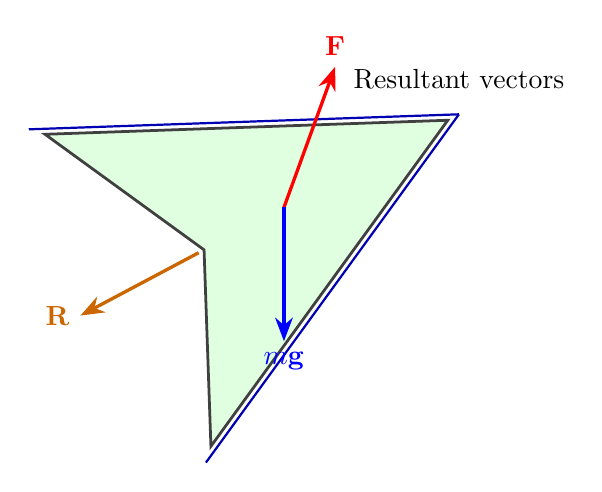
\begin{tikzpicture}[>=Stealth]
  \node[dart,dart tip angle=52,dart tail angle=128,
    shape border uses incircle,shape border rotate=28,
    minimum width=32mm,minimum height=46mm,
    draw=black!75,fill=green!12,line width=1pt,outer sep=2pt] (body) at (0,0) {};
  \draw[blue!70!black,thick] (body.left tail) -- (body.tip);
  \draw[blue!70!black,thick] (body.right tail) -- (body.tip);
  \draw[-{Stealth[length=3mm]},red,line width=1.2pt]
    (body.center) -- ++(70:19mm) node[above] {$\mathbf F$};
  \draw[-{Stealth[length=3mm]},blue,line width=1.2pt]
    (body.center) -- ++(-90:17mm) node[below] {$m\mathbf g$};
  \draw[-{Stealth[length=3mm]},orange!80!black,line width=1.2pt]
    (body.tail center) -- ++(208:17mm) node[left] {$\mathbf R$};
  \node[above=2mm] at (body.tip) {Resultant vectors};
\end{tikzpicture}
\end{document}
